\documentclass[12pt,a4paper]{ctexart}

\usepackage{geometry}
\usepackage{graphicx}
\usepackage{amsmath}
\usepackage{array}
\usepackage{booktabs}
\usepackage{xeCJK}
\usepackage{tikz}
\usepackage{titlesec}

% 页面设置
\geometry{
    top=2.5cm,
    bottom=2.5cm,
    left=2.8cm,
    right=2.8cm
}

% 定义 section* 格式
\titleformat{\section}
  {\zihao{-3}\heiti\bfseries}
  {}
  {0em}
  {}
\titlespacing*{\section}{0pt}{0.5cm}{0.3cm}  % 左缩进、上间距、下间距


% 取消页码（封面）
\pagestyle{empty}

% 定义等长下划线命令（固定宽度 6.5cm，左对齐）
\newcommand{\infofill}[1]{{\zihao{4}\songti\underline{\makebox[6.5cm][c]{#1}}}}

% 定义内容区块命令
\newcommand{\reportsection}[2]{%
    \noindent{\zihao{-3}\heiti\bfseries #1（#2分）}
    \vspace{0.3cm}
    
    \noindent\rule{\textwidth}{0.4pt}
    \vspace{6cm}
}

% 设置中文字体
\setCJKmainfont{SimSun}  % 宋体，可根据系统改为 Noto Serif CJK SC 等

\begin{document}
% ==================== 封面页 ====================
\begin{titlepage}
    \centering
    \vspace*{1.5cm}
    % 校徽占位（正方形示例图）
    
\includegraphics[width=5cm,height=5cm]{images/image-2026-09-07-14-57-04.png}
    
    \vspace{1.8cm}
    
    % 中山大学
    {\zihao{1}\heiti\bfseries 中山大学}
    
    \vspace{0.9cm}
    
    % 微电子科学与技术学院
    {\zihao{2}\heiti 微电子科学与技术学院}
    
    \vspace{0.9cm}
    
    % 课程名称
    {\zihao{2}\heiti 《集成电路元器件特性表征实验》}
    
    \vspace{0.9cm}
    
    % 实验报告
    {\zihao{1}\heiti\bfseries 实验报告}
    
    \vspace{3cm}
    
    % 信息表格
    

    % 信息表格（无任何框线，无横线，无竖线）
    \begin{tabular}{@{}>{\zihao{4}\heiti}r @{\hspace{1.2em}} l@{}}
        实验主题      & \infofill{光传感器的应用探索}        \\[0.8cm]
        姓\quad\quad 名 & \infofill{徐睿琳}   \\[0.8cm]
        学\quad\quad 号 & \infofill{23342107} \\[0.8cm]
        实验日期      & \infofill{\today}   \\[0.8cm]
    \end{tabular}
    
    \vfill
\end{titlepage}

% ==================== 内容页 ====================
\newpage
\pagestyle{plain}
\setcounter{page}{2}

\section*{实验目的（5分）}
\begin{enumerate}
\item 掌握光电容积脉搏波（PPG）的形成机理，理解光传感器将组织血容量变化转换为电信号的过程。
\item 掌握指端脉搏波的采集、脉率计算及对照测量方法，能够分析主要误差来源。
\end{enumerate}

\section*{实验原理（10分）}
LED 照射指端组织后，光经吸收与散射到达探测器。心脏搏动使局部动脉血容量周期性变化，从而调制透射光强：收缩期血容量增大、吸收增强、透射光减弱；舒张期相反，形成近似周期信号。探测器在线性工作区的光电流为
\[
i_{ph}(t)=R_\lambda P(t),
\]
其中 $R_\lambda$ 为波长响应度（A/W），$P(t)$ 为接收光功率（W）；经跨阻放大、滤波与 A/D 转换后得到脉搏波。

采集信号可分解为
\[
s(t)=s_{DC}(t)+s_{AC}(t),
\]
$s_{DC}$ 为非搏动组织与血液形成的背景分量，$s_{AC}$ 反映动脉血容量的搏动变化，脉率信息取自 $s_{AC}$ 的周期。呼吸、运动与环境光会引入干扰；滤波可改善波形但不能消除全部运动伪差。放大电路或软件可能使波形反相，故计数时须取各周期同类特征点。

透射式将 LED 与探测器分置手指两侧，检测穿过组织的光；反射式将二者置于同侧，检测散射回光。两者均可测脉率，单波长即可满足本实验；血氧饱和度尚需多波长信息与标定，本实验不涉及。

在无漏检、无重复计数的连续波段内取 $N$ 个同类主峰，时刻为 $t_1,\ldots,t_N$，则
\[
T=\frac{t_N-t_1}{N-1},\qquad PR=\frac{60}{T},
\]
$PR$ 单位为次/min；宜取至少 4 个连续主峰，若存在缺失峰应另选有效波段。

\section*{实验设备和步骤（5分）}
设备：LED（或手机光源）、硅探测器、同惠 TH1992B 源表及 TonghuiExpert 软件；采用透射式测量。

\begin{enumerate}
\item 源表 sense 端接硅探测器（黑色为正极），食指指腹完全覆盖透光窗口，接触压力以舒适、稳定为准。
\item TonghuiExpert 选择 classic test 下的 I/V-t Sampling：通道 1 或 2，采样间隔 20~ms、采样数 1000、电流范围 100~$\mu$A、偏压 $-0.05$~V；X 轴为时间，Y 轴为电流。
\item 开启光源，静息及运动后各连续记录 20~s、重复 3 次；保存时间戳或采样率、原始信号及测量条件，而非仅记录软件显示值。
\item 去除基线漂移，试用 0.5--5~Hz 带通滤波并剔除边缘不稳定段；标记各周期主峰（每搏仅计一次，排除重搏波、噪声尖峰与运动伪差），按峰间距法计算脉率。
\end{enumerate}


% 导言区需：\usepackage{graphicx,amsmath,booktabs}；中文用 ctex / xeCJK（xelatex 编译）
\section*{实验数据分析（50分）}

\noindent\textbf{1. 数据与预处理。}
三次静息记录取自 TH1992B 源表 I/V-t Sampling：偏压 $-0.05$~V，采样间隔 $20$~ms（$f_s=50$~Hz），每次 $1000$ 点、时长 $19.98$~s，采集时刻为 16:01:46、16:02:48、16:03:29。
原始量 $I_1(t)$ 为负光电流（单位 $\mu$A）。先去除均值（直流基线），再作 $0.5$--$5$~Hz 四阶 Butterworth 零相位带通，得交流分量 $s_{AC}(t)$；剔除首尾不稳定段及第 1 次末端扰动，取 $t\in[1,18]$~s 为有效波段。
因 $I_1=-|I_{ph}|$，收缩期透射光减弱使 $I_1$ 呈正向主峰，故三组均取 $s_{AC}$ 的局部极大作为同类特征点。

\noindent\textbf{2. 波形与峰识别。}
三次原始波形与处理后波形见 Fig.~\ref{fig:wave}，横轴为时间（s）、纵轴为电流（$\mu$A）；第 1 次基线漂移明显，带通后得到抑制。
局部放大见 Fig.~\ref{fig:zoom}，已标出主峰及相邻峰间距 $\Delta t$。峰检测取最小峰距 $0.4$~s、幅度阈值 $0.25\sigma(s_{AC})$，逐段核查重搏波、噪声尖峰与运动伪差，每搏仅计一次主峰，无漏检或重复计数，有效峰数 $N=29$（$\ge 4$，且为连续波段）。

\noindent\textbf{3. 脉率计算与频域校验。}
在连续波段内取 $N$ 个同类主峰，时刻 $t_1,\ldots,t_N$，则
\[
\bar T=\frac{t_N-t_1}{N-1},\qquad PR=\frac{60}{\bar T}\quad(\text{次/min}).
\]
以第 1 次为例：$t_1=1.40$~s，$t_N=17.64$~s，$N=29$，故 $\bar T=0.5800$~s，$PR=103.45$~次/min。三次结果与幅值统计列于 Table~\ref{tab:pr}；峰间期、周期图及脉率对比见 Fig.~\ref{fig:pr}。

\begin{table}[htbp]
\centering
\caption{三次静息 PPG 幅值统计与脉率（峰间距法）}
\label{tab:pr}
\small\setlength{\tabcolsep}{3pt}
\resizebox{\textwidth}{!}{%
\begin{tabular}{lccccccccccc}
\toprule
测量 & $|s_{DC}|$ / $\mu$A & $A_{pp}$ / $\mu$A & $\frac{A_{pp}}{|s_{DC}|}$ / \% & $N$ & $t_1$ / s & $t_N$ / s & $\bar T$ / s & $PR$ / (次/min) & CV$_{\Delta t}$ / \% & $f_0$ / Hz & $PR_f$ / (次/min)\\
\midrule
第1次 & 26.50 & 0.483 & 1.82 & 29 & 1.40 & 17.64 & 0.5800 & 103.45 & 2.65 & 1.721 & 103.27 \\
第2次 & 25.28 & 0.552 & 2.18 & 29 & 1.50 & 17.84 & 0.5836 & 102.82 & 3.96 & 1.691 & 101.44 \\
第3次 & 24.78 & 0.561 & 2.27 & 29 & 1.20 & 17.48 & 0.5814 & 103.19 & 4.58 & 1.685 & 101.07 \\
\midrule
均值$\pm$SD & -- & -- & -- & -- & -- & -- & -- & $\mathbf{103.15\pm0.32}$ & -- & -- & --\\
\bottomrule
\end{tabular}}
\end{table}

三次静息脉率 $\overline{PR}=103.15\pm0.32$~次/min（$\pm$ 为样本标准差），极差 0.63~次/min，相对离散 0.61\%。
周期图主频 $f_0=1.685$--1.721~Hz，换算 $PR_f=101.07$--103.27~次/min，与峰间距法相差 $<2.5\%$；受 $17$~s 有效时长限制，频率分辨率约 $0.06$~Hz（$\approx 3.5$~次/min），故以峰间距法为准。

\begin{figure}[htbp]
\centering
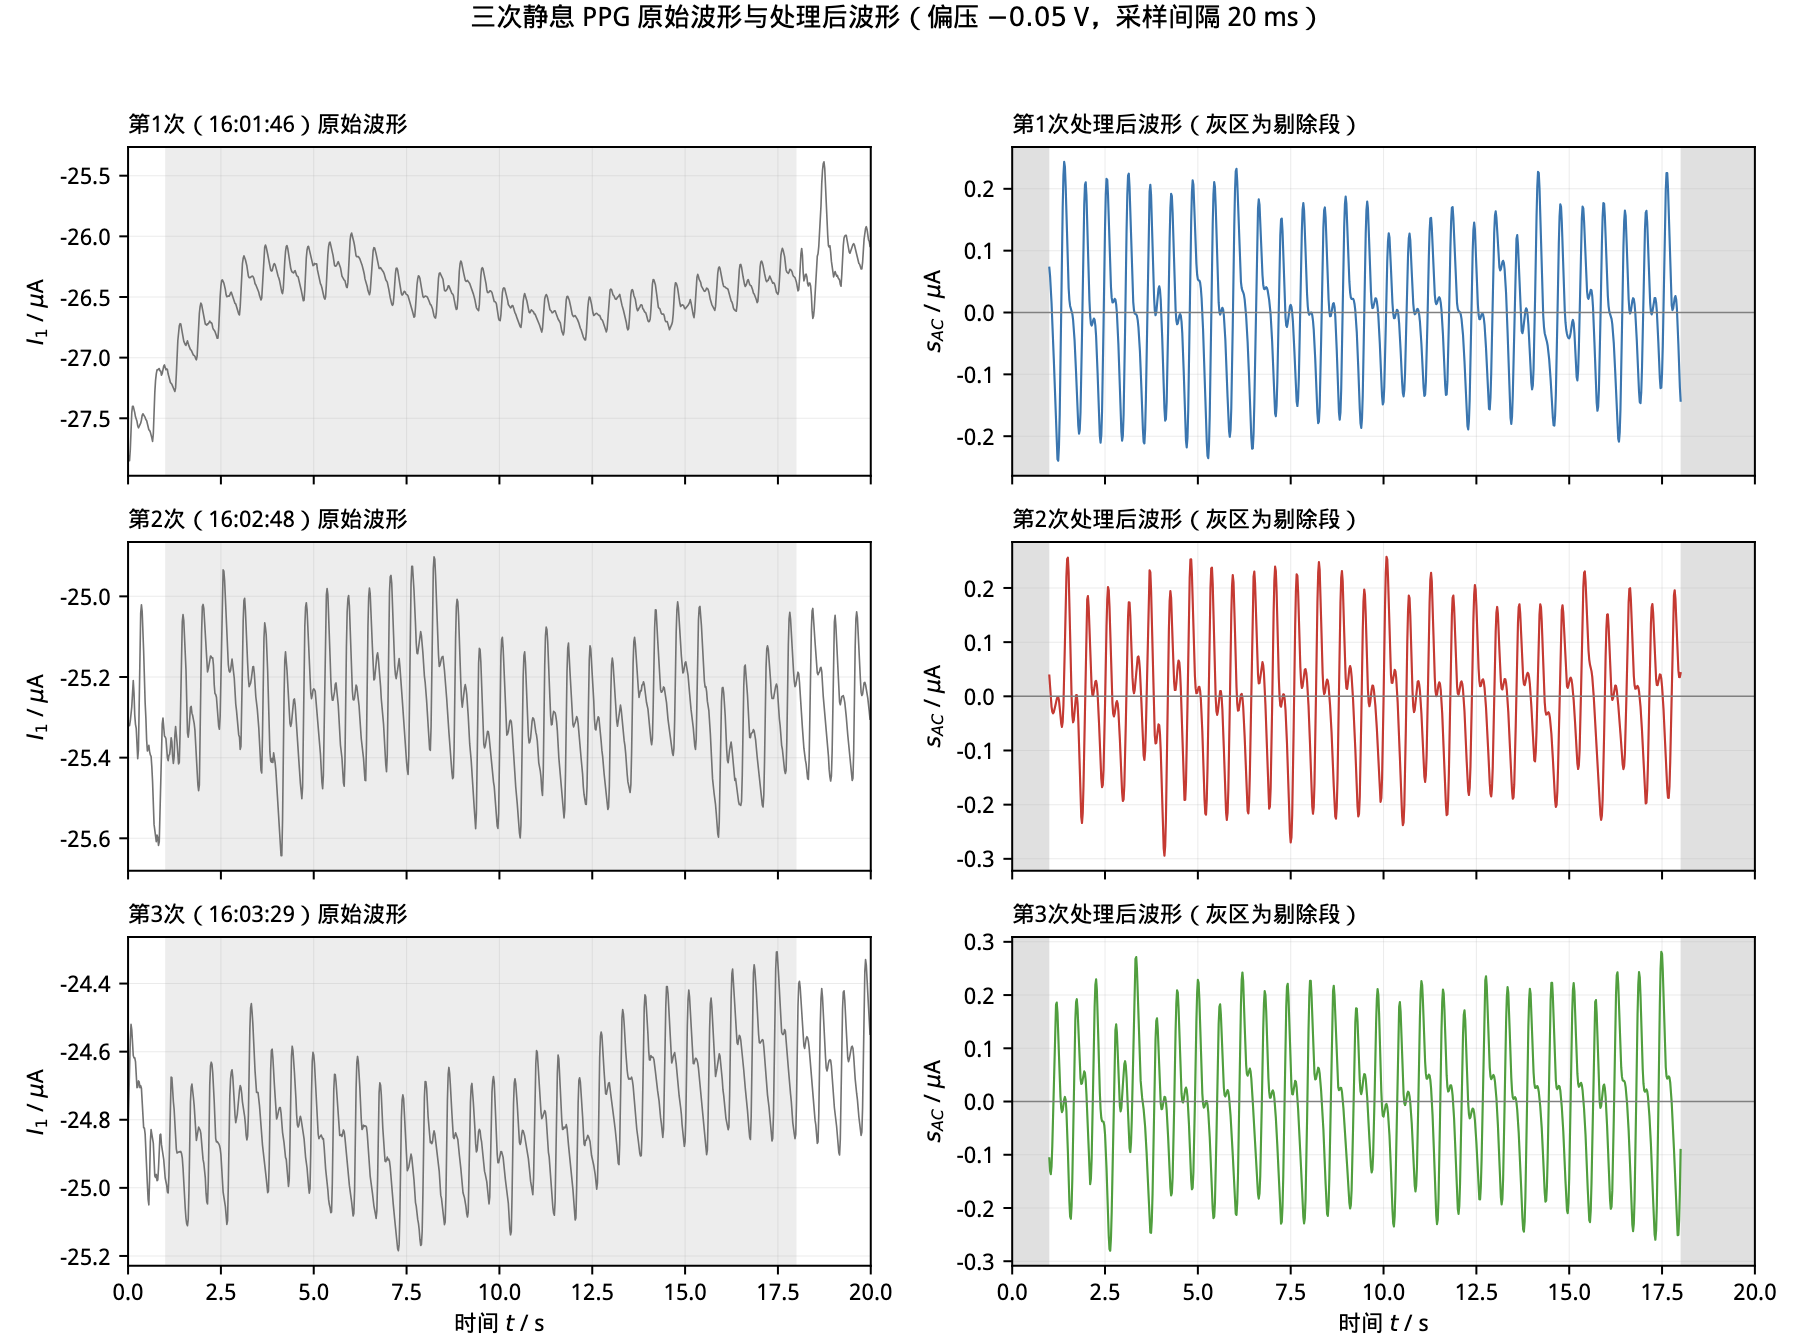
\includegraphics[width=0.98\textwidth]{images/image-2026-11-08-19-33-53.png}
\caption{三次静息原始波形（左，全 $20$~s，浅底为有效波段）与处理后波形（右，仅有效波段，灰区为剔除段）。横轴时间 $t$/s，纵轴电流/$\mu$A；$s_{AC}$ 为 $0.5$--$5$~Hz 带通后的交流分量。}
\label{fig:wave}
\end{figure}

\begin{figure}[htbp]
\centering
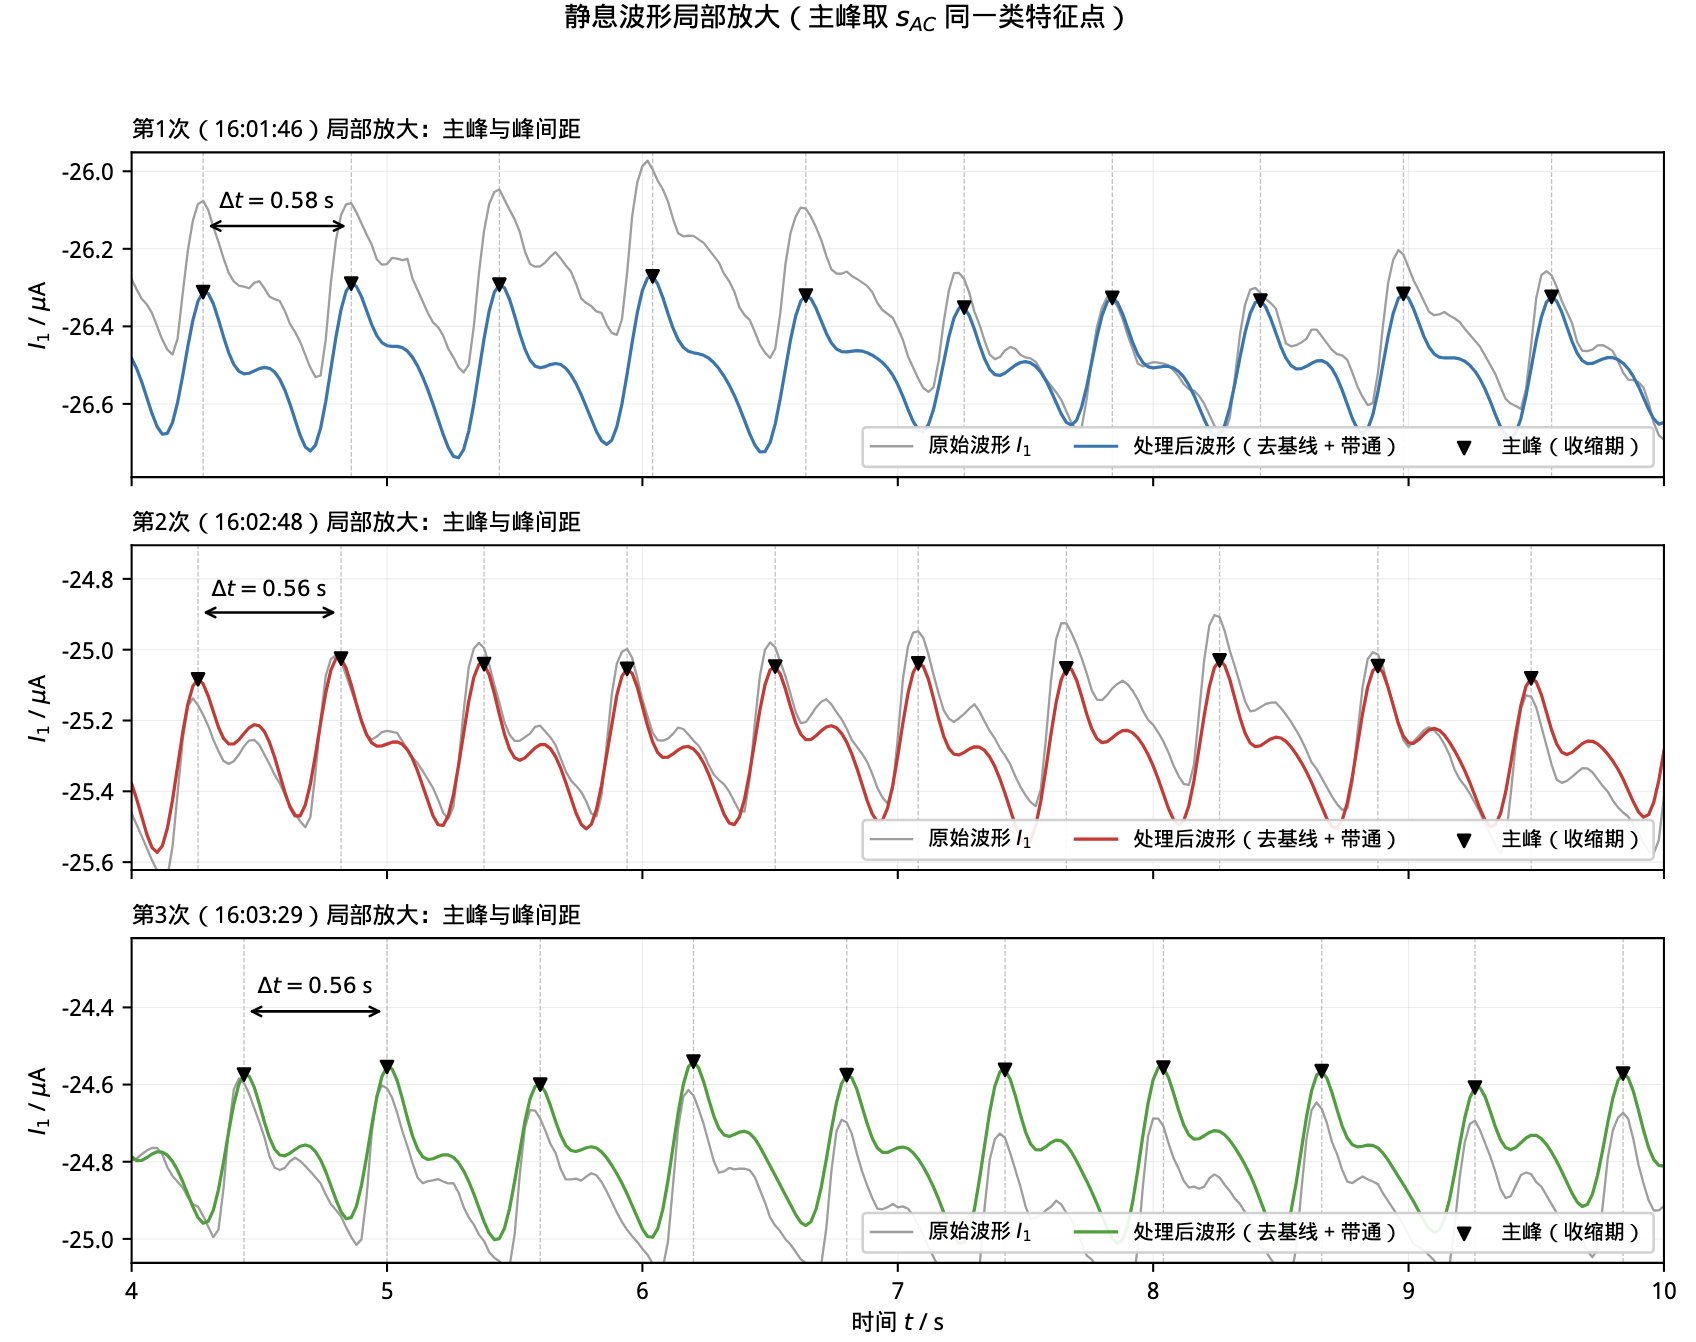
\includegraphics[width=0.88\textwidth]{images/image-2026-11-08-19-34-32.png}
\caption{$4$--$10$~s 局部放大：灰线为原始 $I_1$，彩线为去基线并带通后的波形，倒三角为收缩期主峰，双向箭头标出相邻峰间距 $\Delta t$。横轴时间 $t$/s，纵轴电流/$\mu$A。}
\label{fig:zoom}
\end{figure}

\begin{figure}[htbp]
\centering
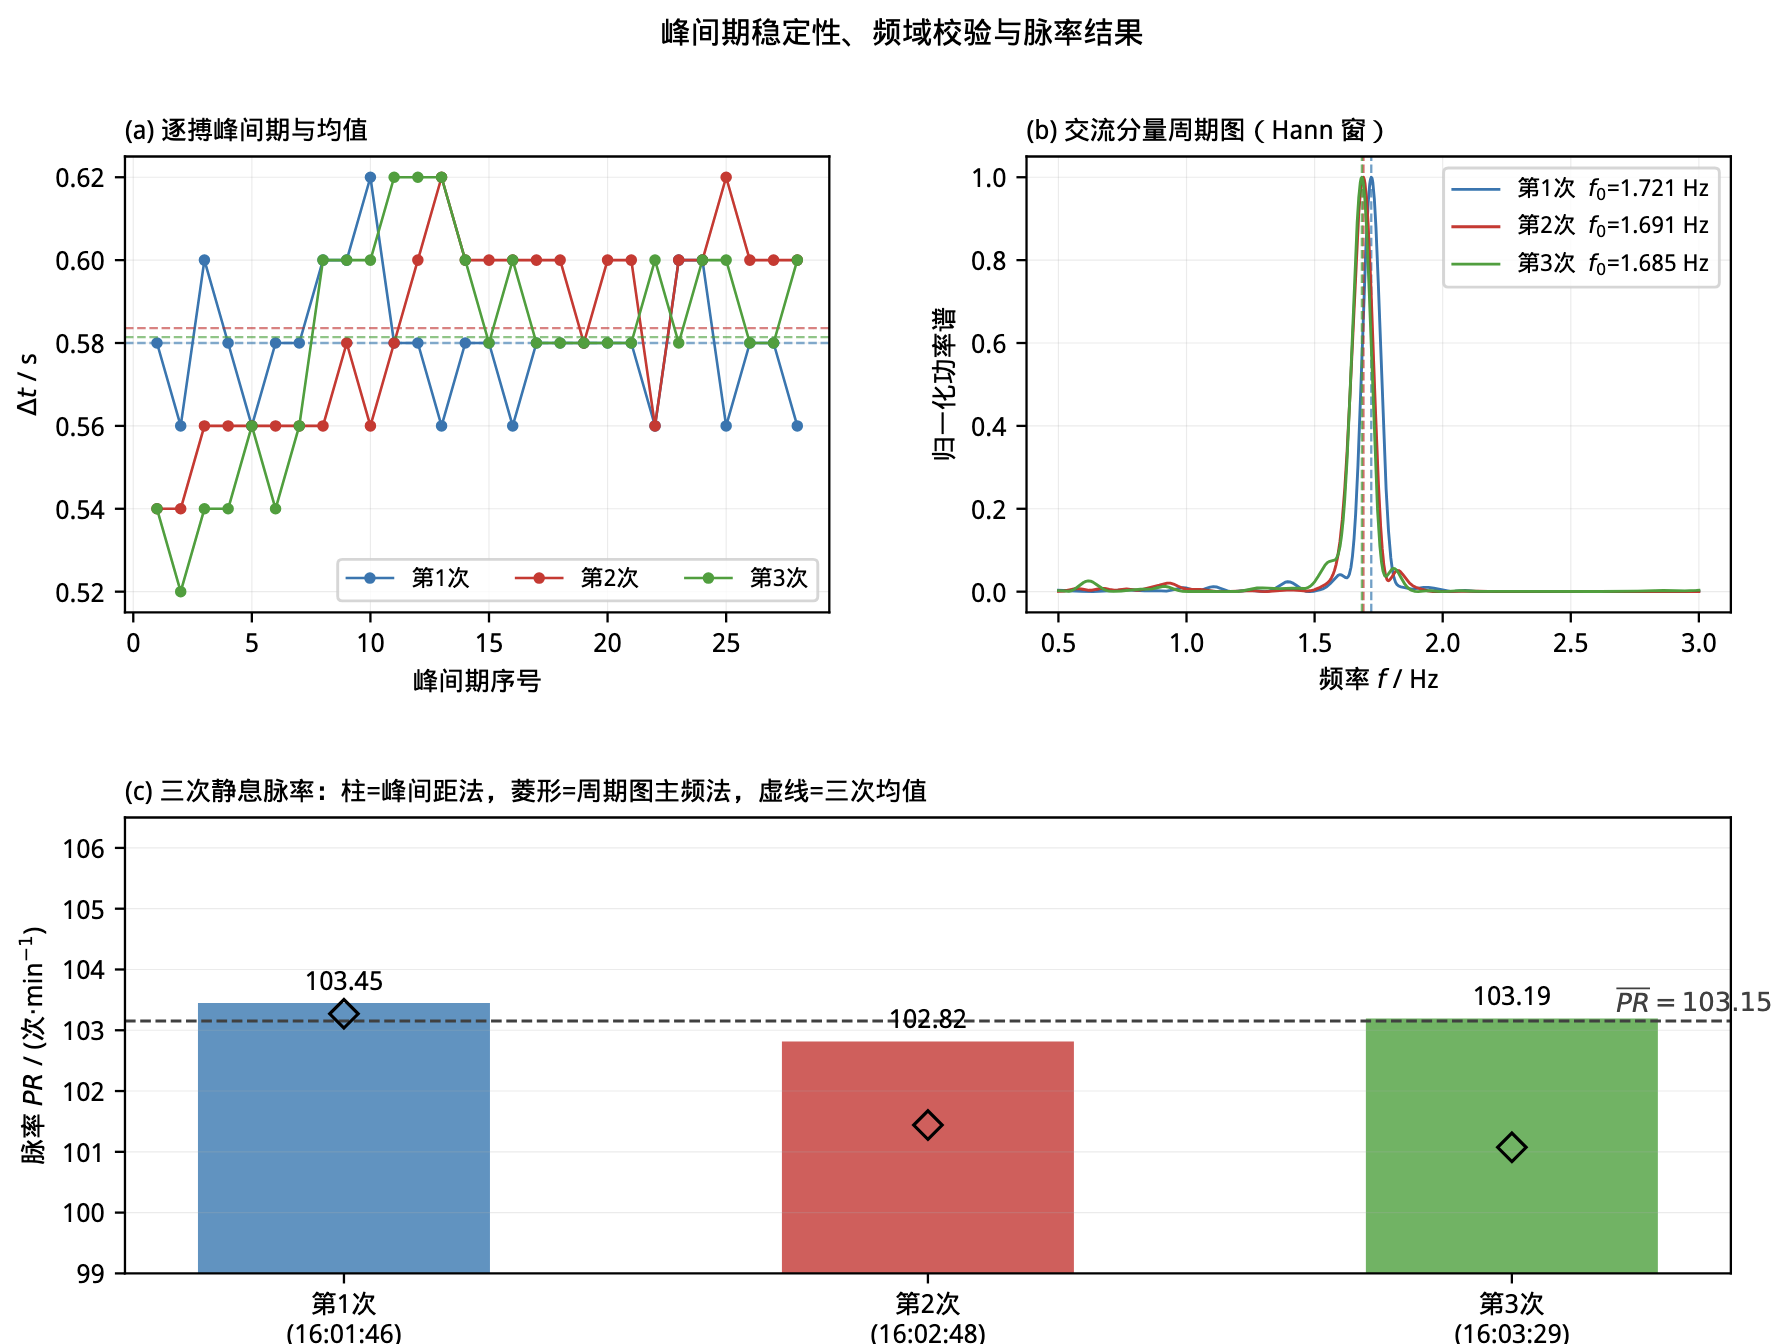
\includegraphics[width=0.94\textwidth]{images/image-2026-11-08-19-34-55.png}
\caption{(a) 逐搏峰间期及其均值；(b) 交流分量归一化周期图，虚线为主频；(c) 三次脉率，柱为峰间距法、菱形为周期图主频法，虚线为三次均值（纵轴自 $99$~次/min 起）。}
\label{fig:pr}
\end{figure}

\noindent\textbf{4. 误差与讨论。}
(1) $|s_{DC}|$ 由 $26.50$ 降至 $24.78$~$\mu$A，$A_{pp}\approx 0.5$~$\mu$A，$A_{pp}/|s_{DC}|\approx 2\%$，符合交流分量远小于直流背景的 PPG 特征；直流缓漂源于手指放置、光源耦合与接触压力变化，不改变搏动周期。
(2) 逐搏峰间期 CV 为 2.65\%--4.58\%，主要来自呼吸性心率变异与轻微位移；多周期平均后三次脉率标准差仅 0.32~次/min。
(3) 主要误差源：接触压力与漏光/环境光、手指微动伪差（第 1 次 $18.5$~s 附近可见尖峰）、带通边缘效应、峰定位量化（$\pm0.01$~s）及重搏波误判。
均值约 $103$~次/min 略高于成人静息常用参考上限，鉴于三次独立记录高度一致且频域结果吻合，应归因于受试者当时状态而非计数错误。
(4) 所给数据仅含 3 次静息记录，未提供运动后波形；实验说明中运动后波形、局部放大图及相应脉率须补测后按同一流程给出。

\noindent\textbf{5. 结论。}
三次静息指端 PPG 周期稳定，峰间距法得静息脉率 $103.15\pm0.32$~次/min；$0.5$--$5$~Hz 带通与同类主峰选取有效抑制基线漂移与伪差，周期图主频提供独立校验。

\section*{实验结论（20分）}
\begin{enumerate}
\item 透射式指端 PPG 将动脉血容量搏动调制为光电流交流分量：实测 $|s_{DC}|\approx 25$~$\mu$A、$A_{pp}\approx 0.5$~$\mu$A，$A_{pp}/|s_{DC}|\approx 2\%$，与 $i_{ph}=R_\lambda P$、$s=s_{DC}+s_{AC}$ 的模型一致。
\item 去基线并作 $0.5$--$5$~Hz 零相位带通后，按同类主峰峰间距法得三次静息脉率 $103.45$、$102.82$、$103.19$~次/min，均值 $103.15\pm0.32$~次/min（极差 $0.63$~次/min）；周期图主频 $1.685$--$1.721$~Hz 给出独立校验（偏差 $<2.5\%$）。
\item 主要误差来自接触压力与漏光、运动伪差、带通边缘效应及峰定位量化（$\pm0.01$~s）；多周期平均与人工核查可将三次离散控制在 $0.61\%$ 以内。本次数据仅含静息记录，运动后结果待补测。
\end{enumerate}

\section*{实验启示和拓展（10分）}
\begin{enumerate}
\item PPG 反映外周容积脉搏，ECG 反映心脏电活动；受脉搏传导时间、外周灌注与心律异常影响，二者波形与计数不可等同，对照测量宜同步记录。
\item 透射式信噪比高而受限于薄组织，反射式可置于腕部更利可穿戴；增加多波长信息并标定后可拓展至血氧饱和度测量。
\item 引入加速度计参考与自适应滤波以抑制运动伪差；控制接触压力、指端温度与环境光，核查波形反相与重搏波，避免重复计数。
\item 可进一步开展运动后恢复曲线、呼吸性心率变异及与商用指夹/心电模块的对照，界定单波长脉率的适用边界。
\end{enumerate}



\end{document}